\section{Übersicht}

\begin{frame}
  {Übersicht}
  \onslide<+->
  \begin{itemize}[<+->]
    \item Silben
    \item Sonorität
    \item Extrasilbizität
    \item Anfangs- und Endrand
    \item Silbengewicht
      \Zeile
    \item Silbengelenke
    \item Schärfungsschreibung als Gelenkschreibung
  \end{itemize}
\end{frame}

\section{Silben}

\begin{frame}
  {Was sind Silben?}
  \pause
  \begin{itemize}[<+->]
    \item genaue Definition schwierig
    \item "`rhythmische Einheiten"' (bzw.\ metrische Einheiten)
      \Zeile
    \item \alert{rein phonologische} Ebene \alert{zwischen Segment und Wort}
    \item eigene \alert{Regularitäten}: Abfolge der Segmente
      \Zeile
    \item \alert{nicht lexikalisch festgelegt}: \textit{klüger} [klyː.g\rot{ɐ}], \textit{klügere} [klyː.g\rot{ə}.\rot{ʁ}ə]
  \end{itemize}
\end{frame}

\begin{frame}[fragile]
  {Silbenstruktur, konstruiert am Einsilbler}
  \pause
  Im Einsilbler:\\
  \begin{itemize}[<+->]
    \item \rot{immer ein Vokal}
    \item \alert{immer mindestens ein Konsonant davor (ggf.\ [ʔ])}
    \item möglicherweise Konsonanten danach\\
      (ohne: \alert{offene} Silbe, mit: \alert{geschlossene} Silbe)
  \end{itemize}
  \Zeile
  \pause
  \begin{center}
    \begin{forest}
      [Silbe, calign=last
        [Anfangsrand, sake, calign=first
          [C][C]
        ]
        [Reim, calign=first
          [Kern, sake, calign=first
            [V]
          ]
          [Endrand, sake, calign=last
            [C][C]
          ]
        ]
      ]
    \end{forest}
  \end{center}
\end{frame}



\begin{frame}[fragile]
  {Sonorität und Sonoritätshierarchie}
  \pause
  \begin{itemize}[<+->]
    \item \textit{Tag}, \textit{Mund}, \textit{Lob}, \textit{Knack}, \textit{grün}, \textit{Klang}, \dots
      \Zeile
    \item Prototypisch:
      \begin{itemize}[<+->]
        \item \alert{Sprechwerkzeuge öffnen und schließen}
        \item \alert{Stimmton geht an und aus.}
      \end{itemize}
      \Zeile
    \item unterschiedliche Öffnungsgrade bei Plosiven, Frikativen,\\
      Nasalen, Liquiden (/ʁ/ /l/), Vokalen korrespondieren mit \alert{Sonorität}
      
  \end{itemize}
  \pause
  \begin{center}
    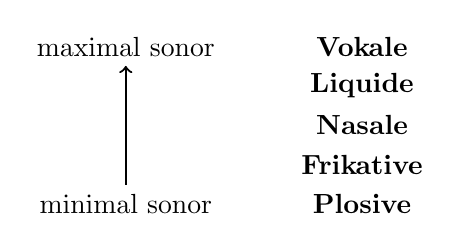
\begin{tikzpicture}
      \node (min)                             {minimal sonor};
      \node (plo) at ([shift={( 3,0)}]   min) {\textbf{Plosive}};
      \node (fri) at ([shift={( 0,0.5)}] plo) {\textbf{Frikative}};
      \node (nas) at ([shift={( 0,0.5)}] fri) {\textbf{Nasale}};
      \node (liq) at ([shift={( 0,0.5)}] nas) {\textbf{Liquide}};
      \node (vok) at ([shift={( 0,0.5)}] liq) {\textbf{Vokale}};
      \node (max) at ([shift={(-3,0)}]   vok) {maximal sonor};
      \draw [->, thick] (min) to (max);
    \end{tikzpicture}
  \end{center}
\end{frame}


\begin{frame}[fragile]
  {Sonoritätskonturen}
  \pause
  \begin{center}
      \SonDiag[2]{{k/\plo/0, u:/\vok/0}}
  \end{center}
\end{frame}

\begin{frame}[fragile]
  {Sonoritätskonturen}
  \begin{center}
      \SonDiag[2]{{n/\nas/0, i:/\vok/0}}
  \end{center}
\end{frame}

\begin{frame}[fragile]
  {Sonoritätskonturen}
  \begin{center}
      \SonDiag[3]{{k/\plo/0, n/\nas/0, i:/\vok/0}}
  \end{center}
\end{frame}

\begin{frame}[fragile]
  {Sonoritätskonturen}
  \begin{center}
      \SonDiag[3]{{d/\plo/0, ʁ/\liq/0, oː/\vok/0}}
  \end{center}
\end{frame}

\begin{frame}[fragile]
  {Sonoritätskonturen}
  \begin{center}
      \SonDiag[3]{{ʃ/\fri/2, t/\plo/0, e:/\vok/0}}
  \end{center}
\end{frame}

\begin{frame}[fragile]
  {Sonoritätskonturen}
  \begin{center}
      \SonDiag[4]{{ʃ/\fri/2, p/\plo/0, ʁ/\liq/0, y:/\vok/0}}
  \end{center}
\end{frame}

\begin{frame}[fragile]
  {Sonoritätskonturen}
  \begin{center}
      \SonDiag[3]{{ʔ/\plo/0, a/\vok/0, p/\plo/0}}
  \end{center}
\end{frame}

\begin{frame}[fragile]
  {Sonoritätskonturen}
  \begin{center}
      \SonDiag[3]{{ʔ/\plo/0, a/\vok/0, n/\nas/0}}
  \end{center}
\end{frame}

\begin{frame}[fragile]
  {Sonoritätskonturen}
  \begin{center}
      \SonDiag[4]{{ʔ/\plo/0, a/\vok/0, χ/\fri/0, t/\plo/0}}
  \end{center}
\end{frame}

\begin{frame}[fragile]
  {Sonoritätskonturen}
  \begin{center}
      \SonDiag[4]{{ʔ/\plo/0, a/\vok/0, l/\liq/0, m/\nas/0}}
  \end{center}
\end{frame}

\begin{frame}[fragile]
  {Sonoritätskonturen}
  \begin{center}
      \SonDiag[4]{{ʁ/\liq/0, a/\vok/0, p/\plo/0, s/\fri/2}}
  \end{center}
\end{frame}



\begin{frame}[fragile]
  {Extrasilbisch}
  \pause
  \begin{itemize}[<+->]
    \item eingekreist: \alert{Verletzungen der Sonoritätskontur}
    \item Lösung: nicht i.\,e.\,S.\ Bestandteile der Silben
    \item \rot{extrasilbische} Konsonanten
      \Zeile
    \item im Anfangsrand nur: \alert{/ʃ/}
    \item im Endrand nur: \alert{/s/ und /t/}
    \item nur \rot{alveolare Obstruenten} (im weiteren Sinn)
      \Zeile
    \item Ist ein Segement extrasilbisch, sind es auch alle folgenden:
  \end{itemize}
  \pause
  \begin{center}
    \SonDiag[6]{{h/\fri/0, ɛ͡ə/\vok/0, p/\plo/0, s/\fri/2, t/\plo/2, s/\fri/2}}
  \end{center}
\end{frame}

\begin{frame}[fragile]
  {Silbenstruktur mit Extrasilbizität}
  \pause
  \begin{center}
  \SonDiag[8]{{ʃ/\fri/2, t/\plo/0, ʁ/\liq/0, ɔ/\vok/0, l/\liq/0, ç/\fri/0, s/\fri/2, t/\plo/2}}
  \Zeile
  \pause
  \begin{forest}
    [Silbe, calign=last
      [Anfangsrand, sake, calign=child, calign child=2
        [X, edge=dashed][C][C]
      ]
      [Reim, calign=first
        [Kern, sake
          [V]
        ]
        [Endrand, sake, calign=child, calign child=2
          [C][C][X,edge=dashed][X,edge=dashed][X,edge=dashed]
        ]
      ]
    ]
  \end{forest}
  \end{center}
\end{frame}


\begin{frame}
  {Was wo steht: Anfangsrand}
  \pause
  \scalebox{0.75}{\begin{minipage}{\textwidth} 
  \begin{exe}
    \ex Simplex
    \pause
    \begin{xlist}
      \ex Po, Bau, Tau, Deich, Kuh, Gang
      \pause
      \ex Fee, Weh, Schuh, hau, Sau, Joch
      \pause
      \ex Mond, Nacht
      \pause
      \ex Lied, Reh
    \end{xlist}
    \pause
    \ex Duplex
    \pause
    \begin{xlist}
      \ex Qual
      \pause
      \ex Knie, Gnu
      \pause
      \ex \alert{Pracht, Bräu, Trank, Dreh, Krach, Grind}
      \pause
      \ex \alert{Fracht, Wrack}
      \pause
      \ex \alert{Platz, Blau, Klang, Glas}
      \pause
      \ex \alert{Floh}
    \end{xlist}
    \pause
    \ex Mit extrasilbischem Konsonanten
    \pause
    \begin{xlist}
      \ex Span, Stau; Spruch, Streich; Spliss
      \pause
      \ex Schwund
      \pause
      \ex Schmach, Schnee
      \pause
      \ex Schlauch, Schrank
    \end{xlist}
  \end{exe}
  \end{minipage}}
\end{frame}


\begin{frame}
  {Was wo steht: Endrand, duplex}
  \pause
  \scalebox{0.85}{\begin{minipage}{\textwidth} 
  \begin{exe}
    \ex Abt, Akt
    \Zeile
    \pause
    \ex Haft, Knast, Acht
    \Zeile
    \pause
    \ex
    \begin{xlist}
      \ex Bank, Rang(?), Hanf, Mensch, Gans
      \pause
      \ex Lump, Ramsch, Wams
    \end{xlist}
    \Zeile
    \pause
    \ex
    \begin{xlist}
      \ex \alert{Korb, Ort, Mark; Alp, Halt, welk}
      \pause
      \ex \alert{Hort, Dorsch, Lurch; Welt, falsch, Milch}
      \pause
      \ex Darm, Kern; Qualm, Köln
    \end{xlist}
  \end{exe}
  \end{minipage}}
  \Zeile
\end{frame}

\begin{frame}
  {Prototypische komplexe Ränder}
  \pause
  \Zeile
  \Large
  \centering
  Der prototypische komplexe Anfangsrand besteht aus\\
  \alert{einem Obstruenten gefolgt von einem Liquid}.\\
  \Zeile
  \pause
  Der prototypische komplexe Endrand besteht aus\\
  \alert{einem Liquid gefolgt von einem Obstruenten}.\\
  \pause
  \Zeile
  Prototypischer komplexer Anfangsrand und Endrand\\
  sind \alert{spiegelbildlich} aufgebaut.
\end{frame}


\begin{frame}
  {Warum reden wir jetzt gleich vom Silbengewicht?}
  \pause
  Wir erfassen zwei wesentliche Beobachtungen:
  \pause
  \Zeile
  \begin{itemize}[<+->]
    \item Es gibt u.\,a.\ Einschränkungen der Besetzungsmöglichkeiten\\
      des \alert{Endrands}, die von der \alert{Länge des Kern-Vokals} abhängen.
    \item Offene Silben mit kurzem Vokal gibt es (fast) nur mit Schwa.
  \Zeile
\item Diese Beschränkung betrifft also den \alert{Reim}.
  \end{itemize} 
\end{frame}

\begin{frame}
  {Silbengewicht als Beschränkung im Reim}
  \pause
  \Halbzeile
  \begin{center}
  \scalebox{0.8}{
  \begin{tabular}{llll}
    \toprule
                         & \textbf{Kern}        & \textbf{Endrand} & \textbf{Beispiele} \\
    \midrule
    \textbf{einmorig}    & \multirow{2}{*}{/ə/} & & \multirow{2}{*}{{}[ʔeː.ə], [tʁuː.ə]} \\
    (überleicht)         &                      & & \\
    \midrule
    \textbf{zweimorig}   & V & C & {}[ʔap], [knap]\\
    (leicht)             & VV & & {}[bla͡ɔ], [ʃneː], \rot{*[ʃne]} \\
    \midrule
    \textbf{dreimorig}   & V & CC & {}[balt], [ʔɪst], [nakt], \rot{*[baːlk]}, \rot{*[ʔiːmʃ]} \\
    (schwer)             & VV & C & {}[zoːk], [la͡ɔp], \rot{*[baːŋk]}, \rot{*[kvaːlm]} \\
    \bottomrule
  \end{tabular}
  }
  \end{center}
  \pause
  \Zeile
  \raggedright
  \begin{itemize}[<+->]
    \item \alert{Nur der \textbf{Reim} ist für das Silbengewicht relevant!}
    \item überleichte (einmorige) Silben nur mit Schwa\ldots\\
      und in speziellen Umgebungen (siehe unten, Korrektur zu EGBD3) \\
    \item überschwere (vier- oder mehrmorige) Silben \rot{niemals} möglich
  \end{itemize}
\end{frame}


% \begin{frame}
%   {Extrasilbisch II}
%   \pause
%   \scalebox{0.85}{\begin{minipage}{\textwidth} 
%   \begin{exe}
%     \ex Nicht überschwer (also max.\ drei Moren):
%     \begin{xlist}
%       \ex /ăçt/ $\Rightarrow$ [ʔaχt] (\textit{Acht})
%       \pause
%       \ex /lɛ̆st/ $\Rightarrow$ [lɛst] (\textit{lässt})
%       \pause
%       \ex /năkt/ $\Rightarrow$ [nakt] (\textit{nackt})
%       \pause
%       \ex /kʁăçs/ $\Rightarrow$ [kʁaχs] (\textit{Krachs})
%       \pause
%       \ex /ăçt/ $\Rightarrow$ [ʔaχt] (\textit{Acht})
%     \end{xlist}
%     \pause
%     \ex Extrasilbizität wegen drohender Überschwere:
%     \begin{xlist}
%       \ex /lest/ $\Rightarrow$ [leːs+t] (\textit{lest})
%       \pause
%       \ex /ʁuft/ $\Rightarrow$ [ʁuːf+t] (\textit{ruft})
%       \pause
%       \ex /huts/ $\Rightarrow$ [huːt+s] (\textit{Huts})
%       \pause
%       \ex /legt/ $\Rightarrow$ [leːk+t] (\textit{legt})
%       \pause
%       \ex /la͡ɔfs/ $\Rightarrow$ [la͡ɔf+s] (\textit{Laufs})
%       \pause
%       \ex /fʊʁçt/ $\Rightarrow$ [fʊ͡əç+t] (\textit{Furcht})
%       \pause
%       \ex /fɛ̆lʃst/ $\Rightarrow$ [fɛlʃ+st] (\textit{fälschst})
%     \end{xlist}
%   \end{exe}
%   \end{minipage}}
% \end{frame}


\begin{frame}
  {Überleichte Silben mit betonbaren Vokalen?}
  \pause
  Was ist mit:
  \begin{itemize}[<+->]
    \item \rot{[bʊ]} in [ˈbʊ.tɐ]
    \item \rot{[ma]} in [ˈma.t͡ʃə]
    \item \rot{[klɪ]} in [ˈklɪ.ŋə]
  \end{itemize}
  \Zeile
  \centering
  \pause
  \rot{Sind das doch einmorige (überleichte) Silben mit Vollvokal?}\\
  \Zeile
  \pause
  \raggedright
  Dieser Silbentyp tritt nur auf:\\
  \begin{itemize}[<+->]
    \item \alert{in (scheinbar) offenen Silben} (sonst nicht überleicht)
    \item \alert{in der betonten Silbe eines Trochäus}
    \item \alert{vor simplexen Anfangsrändern}
  \end{itemize}
\end{frame}

\begin{frame}
  {Silbengelenke}
  \pause
  Lösung: Die Silben sind \alert{nicht überleicht}, \alert{der Konsonant\\
  an der Silbengrenze gehört zum Endrand der ersten und\\
zum Anfangsrand der zweiten Silbe}.\\
  \pause
  \Zeile
  \begin{center}
  \begin{forest}
    [Wort
      [Silbe, calign=last
        [Anfangsrand, ake
          [m]
        ]
        [Reim, calign=first
          [Kern, ake
            [ɪ]
          ]
          [Endrand, ake, name=ERBaum]
        ]
      ]
      [Silbe, calign=last
        [Anfangsrand, ake
          [t]
          {\draw[-] (.north) -- (ERBaum.south);}
        ]
        [Reim
          [Kern, ake
            [ə]
          ]
        ]
      ]
    ]
  \end{forest}
  \end{center}
\end{frame}

\begin{frame}
  {Silbengelenke}
  \begin{center}
  \SonDiag[4]{{m/\nas/0, ɪ/\vok/0, t/\plo/1, ə/\vok/0}}    
  \end{center}
\end{frame}




\section{Schärfung}


\begin{frame}
  {Das Faszinosum der Schärfungsschreibung}
  \pause
  Dehnungs-\slash Schärfungsschreibungen (Einsilbler\slash trochäischer Zweisilbler)\\
  \Zeile
  \pause
  \centering
  \resizebox{0.85\textwidth}{!}{
    \begin{tabular}{lllllllll}
      \toprule
      & & & \textbf{ɪ} & \textbf{ʊ} & \multicolumn{2}{l}{\LocStrutGrph\textbf{ɛ̆}} & \textbf{ɔ} & \textbf{ă} \\
      \midrule

      \multirow{4}{*}{\rotatebox{90}{\textbf{ungespannt}}}

      & \multirow{2}{*}{\rotatebox{90}{\textbf{offen}}}
      & \textbf{einsilb.}  & \textit{\Nono}  & \textit{\Nono}           & \multicolumn{2}{l}{\LocStrutGrph\textit{\Nono}}         & \textit{\Nono}        & \textit{\Nono}           \\
      && \textbf{zweisilb.}  & \textit{Li.\alert{pp}e} & \textit{Fu.\alert{tt}er}         & \multicolumn{2}{l}{\LocStrutGrph\textit{We.\alert{ck}e}}        & \textit{o.\alert{ff}en}       & \textit{wa.\alert{ck}er}         \\
        & \multirow{2}{*}{\rotatebox{90}{\textbf{gesch.}}}
        & \textbf{einsilb.}  & \textit{Ki\rot{nn}}   & \textit{Schu\rot{tt}}    & \multicolumn{2}{l}{\LocStrutGrph\textit{Be\rot{tt}}}           & \textit{Ro\rot{ck}}         & \textit{Wa\rot{tt}}            \\
        && \textbf{zweisilb.}  & \textit{Rin.de} & \textit{Wun.der}        & \multicolumn{2}{l}{\LocStrutGrph\textit{Wen.de}}        & \textit{pol.ter}      & \textit{Tan.te}          \\

      \midrule

      \multirow{4}{*}{\rotatebox{90}{\textbf{gespannt}}}

      & \multirow{2}{*}{\rotatebox{90}{\textbf{offen}}}
        & \textbf{einsilb.}  & \textit{Knie}   & \textit{Schuh}       & \textit{Schnee, Reh}  & \textit{zäh}          & \textit{roh}          & (\textit{da})            \\
      && \textbf{zweisilb.}  & \textit{Bie.ne} & \textit{Kuh.le, Schu.le} & \textit{we.nig}       & \textit{Äh.re, rä.kel} & \textit{oh.ne, O.fen} & \textit{Fah.ne, Spa.ten} \\

      & \multirow{2}{*}{\rotatebox{90}{\textbf{gesch.}}}
        & \textbf{einsilb.}  & \textit{lieb}  & \textit{Ruhm, Glut}      & \textit{Weg}          & \textit{spät}           & \textit{rot}          & \textit{Tat}             \\
      && \textbf{zweisilb.}  & (\textit{lieb.lich}) & (\textit{lug.te})   & (\textit{red.lich})   & (\textit{wähl.te})     & (\textit{brot.los})   & (\textit{rat.los})       \\

      \midrule
      & & & \textbf{i} & \textbf{u} & \textbf{e} & \textbf{ε} & \textbf{o} & \textbf{a} \\

      \bottomrule
    \end{tabular}
  }
  \Halbzeile\pause
  \begin{itemize}[<+->]
    \item \alert{Schärfungsschreibung im Trochäus nur nach ungespanntem Vokal\\
      in offener Silbe, wenn Anfangsrand der Zweitsilbe konsonantisch}
    \item \ldots\ \rot{und im geschlossenen Einsilbler mit ungespanntem Vokal}
  \end{itemize}
\end{frame}

\begin{frame}
  {Details und oft Übersehenes}
  \pause
  \begin{itemize}[<+->]
    \item \alert{Schärfungsschreibung = Silbengelenkschreibung}
    \item Aber warum dann im Einsilbler (\textit{Kinn}, \textit{Bett}, \textit{Rock})?
      \begin{itemize}[<+->]
        \item Siehe nächste Woche!
      \end{itemize}
      \Halbzeile
    \item Merke: Silbengelenkschreibung nur da, wo auch Silbengelenk:
      \begin{itemize}[<+->]
        \item \alert{zwischen Erst- und Zweitsilbe des Trochäus}
        \item \alert{nach ungespanntem} (=kurzem) \alert{Vokal}
      \end{itemize}
  \end{itemize}
\end{frame}

\begin{frame}
  {Details und oft Übersehenes II}
  \pause
  \begin{itemize}[<+->]
    \item \alert{keine Schärfungsschreibung bei Di- und Trigraphen}
      \begin{itemize}[<+->]
        \item \textit{Esche} [ɛʃ̣ə], \textit{zischen} [t͡sɪʃ̣ən]
        \item \textit{Kachel} [kaχ̣əl], \textit{Zeche} [t͡sɛç̣ə]
        \item \textit{Kringel} [kʁɪŋ̣əl], \textit{Zunge} [t͡sʊŋ̣ə]
      \end{itemize}
      \Halbzeile
    \item \rot{Warum sind stimmhafte Obstruenten im Silbengelenk "`eigentlich"' unmöglich?}
      \begin{itemize}[<+->]
        \item Obstruent auch im Endrand der Erstsilbe: \alert{Endrand-Desonorisierung}
        \item \textit{Kladde}, \textit{Robbe}, \textit{Bagger}, ?\textit{prasseln} [pʁazəln], *\textit{quivveln}
        \item \ldots\ \rot{nicht Kern} (fünf oder sechs Typen, alle niederdeutsch)
      \end{itemize}
  \end{itemize}
\end{frame}

\begin{frame}
  {Überblick über Gelenkschreibungen}
  \onslide<+->
  \onslide<+->
  \centering 
  \scalebox{0.7}{%
  \begin{tabular}{lllll}
    /k/  & k      & \rot{ck}        & \textit{Macke} & [maḳə] \\
    /t/  & t      & \alert{tt}      & \textit{Matte} & [maṭə] \\
    /p/  & p      & \alert{pp}      & \textit{Mappe} & [map̣ə] \\
      &&&\\
    /t͡ʃ/ & tsch ? & \orongsch{tsch} & \textit{Ratsche} & [ʁaṭ͡ʃə] \\
    /t͡s/ & z      & \rot{tz}        & \textit{platzen} & [plat͡sən] \\
    /p͡f/ & pf     & \orongsch{pf}   & \textit{zupfen} & [t͡sʊp͡f̣ən] \\
      &&&\\
    /χ/  & ch     & \orongsch{ch}   & \textit{Bache} & [baχ̣ə] \\
    /r/  & r      & \alert{rr}      & \textit{Knarre} & [knaʁ̣ə] \\
    /ʃ/  & sch    & \orongsch{sch}  & \textit{Esche} & [ʔɛʃ̣ə] \\
    /s/  & s      & \alert{ss}      & \textit{lassen} & [laṣən] \\
    /f/  & f      & \alert{ff}      & \textit{hoffen} & [hɔf̣ən] \\
      &&&\\
    /n/  & n      & \alert{nn}      & \textit{Wanne} & [vaṇə] \\
    /m/  & m      & \alert{mm}      & \textit{Kämme} & [kɛṃə] \\
    /l/  & l      & \alert{ll}      & \textit{knallen} & [knaḷən] \\
      &&&\\
    \grau{/g/} &&&& \\
    \grau{/d/} &&&& \\
    \grau{/b/} &&&& \\
  \end{tabular}%
}
\end{frame}



\ifdefined\TITLE
  \section{Nächste Woche | Überblick}

  \begin{frame}
    {Semesterplan}
    \begin{enumerate}
      \item Graphematik und Schreibprinzipien
      \item Wiederholung -- Phonetik
      \item Wiederholung -- Phonologie
      \item Phonographisches Schreibprinzip -- Konsonanten
      \item Phonographisches Schreibprinzip -- Vokale
      \item Silben und Dehnungsschreibungen
      \item \alert{Eszett, Dehnung und Konstanz}
      \item Spatien und Majuskeln
      \item Komma
      \item Punkt und sonstige Interpunktion
    \end{enumerate}
  \end{frame}
\fi
